% Provenance (never printed): see sources/outline_sources.md (Year 1:
% the Solar System, planetology). Kepler's laws, the moment of inertia and
% the Stefan--Boltzmann law are owned by the physics series and recalled
% here; the equilibrium temperature and the Bond albedo are re-founded from
% Book 2 grade 10. Curves computed in figdata/bachelor-1/planet_table.py;
% numbers of the exercises and problem in the Book 3 scratch calculator
% ch03.py.
\chapter{तुलनात्मक ग्रह विज्ञान}\label{ch:b1:comparative-planetology}

शुक्र और पृथ्वी लगभग जुड़वाँ हैं: शुक्र की त्रिज्या पृथ्वी की \qty{95}{\percent} और द्रव्यमान उसका
\qty{81}{\percent} है। फिर भी पृथ्वी पर महासागर हैं, नाइट्रोजन-ऑक्सीजन वायुमंडल है और चलती प्लेटें हैं,
जबकि शुक्र बादलों के नीचे \qty{737}{K} की सतह छिपाए है, जो किसी भी रसोई के ओवन से गर्म है, और
\qty{92}{bar} पर एक कार्बन-डाइऑक्साइड वायुमंडल से दबी है। मंगल, पृथ्वी के आधे आकार का, पतला और
ठंडा वायुमंडल, विशाल ज्वालामुखी और घाटियाँ रखता है, पर उसकी कोई चलती प्लेट नहीं है। और दूर,
बृहस्पति और शनि मुख्यतः हाइड्रोजन और हीलियम हैं; अरुण और वरुण मुख्यतः जल, मीथेन और अमोनिया की
हिम हैं। ग्रहों की तुलना ही वह एकमात्र तरीका है जिससे यह परखा जा सकता है कि हम पृथ्वी के बारे में
जो जानते हैं वह कितना सच है: उसका भीतरी भाग परतों में क्यों है, उसकी जलवायु सौम्य क्यों है, और
वही क्यों अकेली प्लेट विवर्तनिकी रखती है। यह अध्याय ग्रहों को तौलता और मापता है, उनके घनत्वों और
उनके द्रव्यमान के वितरण से उनके भीतरी भागों को पढ़ता है, उनके तापमानों और वायुमंडलों की तुलना करता
है, और उन चंद्रमाओं और छोटे पिंडों के साथ समाप्त होता है जो सौरमंडल की युवावस्था का अभिलेख रखते हैं।
% ledger: nasa:venus, earth:Rmean, earth:mass, nasa:uranus-structure

\begin{recall}
ग्रह दीर्घवृत्तों पर सूर्य के चारों ओर घूमते हैं, और किसी उपग्रह के आवर्तकाल का वर्ग उसके
अर्ध-दीर्घ अक्ष के घन के समानुपाती होता है (केप्लर का तीसरा नियम, भौतिकी की प्रथम-वर्ष की पुस्तक
में, जहाँ किसी ठोस का जड़त्व-आघूर्ण भी परिभाषित है; एक समान गोले का $I = \tfrac25MR^2$ है)। एक
कृष्णिका प्रति इकाई क्षेत्रफल $\sigma T^4$ विकिरित करती है (दूसरा वर्ष)। सौरमंडल और उसके \omterm{def:b1:comparative-planetology:planet-types}{शैल-ग्रह}
तथा \omterm{def:b1:comparative-planetology:planet-types}{विशाल ग्रह} पुस्तक 1 (कक्षा 6) में वर्णित हुए थे; किसी ग्रह का एल्बिडो और उसका \omterm{def:b1:comparative-planetology:equilibrium-temperature}{साम्य तापमान}
पुस्तक 2 (कक्षा 10) में आए थे, और हरितगृह प्रभाव पुस्तक 1 (कक्षा 9) में।
\end{recall}

\begin{omfigure}
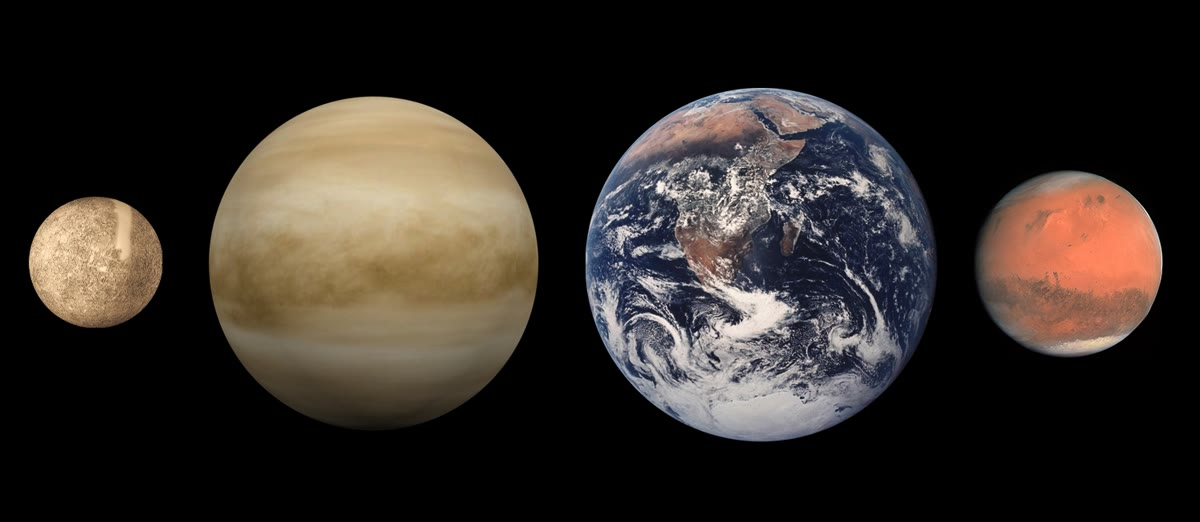
\includegraphics[width=0.85\linewidth]{images/book3/b1-terrestrial-planet-sizes.jpg}

{\small चार \omterm{def:b1:comparative-planetology:planet-types}{शैल-ग्रह} पैमाने पर, बाएँ से दाएँ बुध, शुक्र, पृथ्वी और मंगल (दूरियाँ पैमाने पर नहीं; शुक्र
दृश्य प्रकाश में, जैसा वह दिखता है, उसकी सतह बादलों के नीचे छिपी है)। NASA, सार्वजनिक क्षेत्र।}
% ledger: commons:terrestrial-sizes
\end{omfigure}

\section{ग्रहों को तौलना और मापना}

किसी ग्रह की त्रिज्या उसके कोणीय व्यास और दूरी से मापी जाती है, या, अंतरिक्ष यान द्वारा गए ग्रह के
लिए, रडार और लेज़र ऊँचाई-मापन से। उसका द्रव्यमान कठिन है: वह केवल उस गुरुत्व से अनुभव होता है जो ग्रह
किसी दूसरी वस्तु पर लगाता है।

\begin{method}[उपग्रह की कक्षा से ग्रह का द्रव्यमान]\label{met:b1:comparative-planetology:mass}
नगण्य द्रव्यमान के एक उपग्रह की, लगभग वृत्ताकार कक्षा में, त्रिज्या (अर्ध-दीर्घ अक्ष) $a$ और
नाक्षत्र आवर्तकाल $T$ के लिए, द्रव्यमान $M$ के एक ग्रह के चारों ओर:
\begin{enumerate}
  \item $a$ को मीटर में और $T$ को सेकंड में बदलिए;
  \item केप्लर का तीसरा नियम $GM = 4\pi^2a^3/T^2$ देता है: यह गुणनफल है जो कक्षा मापती है, और $G$ स्वयं
        से कहीं अधिक सूक्ष्मता से;
  \item $G = \qty{6.6743e-11}{m^3.kg^{-1}.s^{-2}}$ से भाग देकर $M$ पाइए।
\end{enumerate}
जिस ग्रह का कोई चंद्रमा नहीं (बुध, शुक्र), उसे उसी प्रकार उस अंतरिक्ष यान की कक्षा, या उसके विचलन से
तौला जाता है जो उसके पास से गुज़रता है।
\end{method}

\begin{example}
बृहस्पति का सबसे भीतरी बड़ा चंद्रमा, आयो, $a = \qty{421.8e3}{km}$ पर \num{1.769138} दिनों में परिक्रमा
करता है, अर्थात् $T = \qty{152854}{s}$। तब
\[
  GM = \frac{4\pi^2\times(\qty{4.218e8}{m})^3}{(\qty{152854}{s})^2}
  = \qty{1.268e17}{m^3.s^{-2}}, \qquad
  M = \frac{\num{1.268e17}}{\num{6.6743e-11}} = \qty{1.900e27}{kg},
\]
जो बृहस्पति के सारणीबद्ध द्रव्यमान, \qty{1.898e27}{kg}, से \qty{0.1}{\percent} के भीतर मेल खाता है।
आयो का अपना द्रव्यमान, बृहस्पति का \num{4.7e-5}, नगण्य है; छोटा आधिक्य बृहस्पति के विषुवतीय
उभार से आता है, जो एक निकट चंद्रमा को उसी द्रव्यमान के गोले से थोड़ा अधिक खींचता है।
% ledger: nasa:io, nasa:jupiter, const:G
\end{example}

द्रव्यमान और त्रिज्या के साथ माध्य घनत्व $\bar\rho =
3M/(4\pi R^3)$ आता है, जो इसका पहला संकेत है कि ग्रह किस चीज़ से बना है। ग्रहों के घनत्व दो समूहों
में पड़ते हैं (नीचे की आकृति देखिए): बुध, शुक्र, पृथ्वी और मंगल लगभग \num{3900} और
\qty{5500}{kg.m^{-3}} के बीच हैं, किसी भी सामान्य चट्टान से सघन; बाहरी चार ग्रह \num{690} और
\qty{1640}{kg.m^{-3}} के बीच हैं, पानी के घनत्व के निकट, और शनि तो उससे भी नीचे।
% ledger: planet:Mercury.density, planet:Mars.density, planet:Earth.density, planet:Saturn.density, planet:Neptune.density

\begin{omfigure}
\begin{tikzpicture}
\begin{axis}[omrecord, width=0.86\linewidth, height=6.2cm, xmode=log,
  xmin=800, xmax=150000, ymin=0, ymax=6300, xlabel={विषुवतीय त्रिज्या (km)},
  ylabel={मध्य घनत्व (\unit{kg.m^{-3}})}, tick label style={font=\scriptsize},
  label style={font=\small}]
\addplot[only marks, mark=*, mark size=2.4pt, brown!70!black] table[x=R_km, y=density,
  restrict expr to domain={\thisrow{idx}}{0:2}] {figdata/out/bachelor-1-planet_table-bodies.dat};
\addplot[only marks, mark=*, mark size=2.4pt, brown!70!black] table[x=R_km, y=density,
  restrict expr to domain={\thisrow{idx}}{4:4}] {figdata/out/bachelor-1-planet_table-bodies.dat};
\addplot[only marks, mark=*, mark size=2.4pt, orange!85!black] table[x=R_km, y=density,
  restrict expr to domain={\thisrow{idx}}{5:6}] {figdata/out/bachelor-1-planet_table-bodies.dat};
\addplot[only marks, mark=*, mark size=2.4pt, omDef] table[x=R_km, y=density,
  restrict expr to domain={\thisrow{idx}}{7:8}] {figdata/out/bachelor-1-planet_table-bodies.dat};
\addplot[only marks, mark=o, mark size=2.4pt, black!60] table[x=R_km, y=density,
  restrict expr to domain={\thisrow{idx}}{3:3}] {figdata/out/bachelor-1-planet_table-bodies.dat};
\addplot[only marks, mark=o, mark size=2.4pt, black!60] table[x=R_km, y=density,
  restrict expr to domain={\thisrow{idx}}{9:9}] {figdata/out/bachelor-1-planet_table-bodies.dat};
\addplot[black!40, densely dashed] coordinates {(800,1000) (150000,1000)};
\begin{scope}[font=\scriptsize]
\node[left] at (axis cs:2439.5,5429) {बुध};
\node[below left] at (axis cs:6052,5243) {शुक्र};
\node[above] at (axis cs:6378,5514) {पृथ्वी};
\node[left] at (axis cs:3396,3934) {मंगल};
\node[left] at (axis cs:1737.5,3340) {चंद्रमा};
\node[right] at (axis cs:1188,1850) {प्लूटो};
\node[above] at (axis cs:71492,1326) {बृहस्पति};
\node[left] at (axis cs:60268,687) {शनि};
\node[right] at (axis cs:25559,1270) {अरुण};
\node[above] at (axis cs:24764,1638) {वरुण};
\node[above left, black!60] at (axis cs:150000,1000) {जल};
\end{scope}
\end{axis}
\end{tikzpicture}

{\small आठ ग्रहों के लिए (भरे: \omterm{def:b1:comparative-planetology:planet-types}{शैल-ग्रह}, \omterm{def:b1:comparative-planetology:planet-types}{गैस दानव}, \omterm{def:b1:comparative-planetology:planet-types}{हिम दानव}), चंद्रमा और प्लूटो (खुले वृत्त)
के माध्य घनत्व बनाम त्रिज्या (लघुगणकीय)। आँकड़े NASA की ग्रह तथ्य-पत्रिका के हैं।}
% ledger: planet:Mercury.diameter, planet:Venus.diameter, planet:Earth.diameter, planet:Moon.diameter, planet:Mars.diameter, planet:Jupiter.diameter, planet:Saturn.diameter, planet:Uranus.diameter, planet:Neptune.diameter, planet:Pluto.diameter, planet:Mercury.density, planet:Venus.density, planet:Earth.density, planet:Moon.density, planet:Mars.density, planet:Jupiter.density, planet:Saturn.density, planet:Uranus.density, planet:Neptune.density, planet:Pluto.density
\end{omfigure}

केवल माध्य घनत्व यह नहीं बता सकता कि ग्रह एक ही सघन पदार्थ का बना है, या उसका बहुत सघन क्रोड और
हल्का आवरण है। एक दूसरी संख्या यह बताती है: द्रव्यमान क्रोड और सतह के बीच कैसे बँटा है।

\begin{definition}[जड़त्व-आघूर्ण गुणक]\label{def:b1:comparative-planetology:moi}
किसी ग्रह का \emph{जड़त्व-आघूर्ण गुणक}\index{जड़त्व-आघूर्ण गुणक} यह संख्या है
\[
  C = \frac{I}{MR^2} ,
\]
जहाँ $I$ उसके घूर्णन अक्ष के परितः उसका जड़त्व-आघूर्ण है, $M$ उसका द्रव्यमान और $R$ उसकी माध्य
त्रिज्या। एक समान गोले के लिए $C = \tfrac25 = 0.4$ है; वह ग्रह जिसका घनत्व केंद्र की ओर बढ़ता है,
उसका $C < 0.4$ है, और यह जितना छोटा होगा, द्रव्यमान उतना ही अधिक केंद्रित होगा।
\end{definition}

जड़त्व-आघूर्ण घूर्णन अक्ष की सूर्य के खिंचाव से होने वाली धीमी अग्रगति से, और ग्रह के गुरुत्व क्षेत्र
के चपटेपन के साथ, मापा जाता है। मान रोचक हैं: चंद्रमा, $C = 0.394$, लगभग एकसमान है; मंगल, $0.366$,
और पृथ्वी, $0.3308$, स्पष्ट रूप से परतदार हैं; बृहस्पति, $0.254$, और शनि, $0.210$, के अधिकांश
द्रव्यमान उनके केंद्रों की ओर सिमटे हैं।
% ledger: nasa:moon, nasa:mars, earth:MoI, nasa:jupiter, nasa:saturn

\section{ग्रह किस चीज़ से बने हैं}

\begin{definition}[शैल-ग्रह और विशाल ग्रह]\label{def:b1:comparative-planetology:planet-types}
एक \emph{शैल-ग्रह}\index{शैल-ग्रह} ऐसा ग्रह है जो मुख्यतः सिलिकेट चट्टान और लोहे से बना है, जिसकी
एक ठोस सतह है: बुध, शुक्र, पृथ्वी और मंगल। एक \emph{विशाल ग्रह}\index{विशाल ग्रह} ऐसा ग्रह है जो
पृथ्वी से कई गुना भारी है, मुख्यतः हल्के तत्वों और उनके यौगिकों से बना है, और उसकी कोई ठोस सतह नहीं
है। एक \emph{गैस दानव}\index{गैस दानव} मुख्यतः हाइड्रोजन और हीलियम से बना विशाल ग्रह है: बृहस्पति
और शनि। एक \emph{हिम दानव}\index{हिम दानव} मुख्यतः उन यौगिकों से बना विशाल ग्रह है जिन्हें
खगोलविद हिम कहते हैं --- जल, मीथेन और अमोनिया --- जो हाइड्रोजन और हीलियम के आवरण के नीचे हैं:
अरुण और वरुण।
\end{definition}

ग्रहों के पास जाने वाले यानों और दूरबीनों से मापे गए वायुमंडल इस विभाजन की पुष्टि करते हैं।
बृहस्पति का आयतन के अनुसार \qty{89.8}{\percent} हाइड्रोजन और \qty{10.2}{\percent} हीलियम है, शनि का
\qty{96.3}{\percent} और \qty{3.25}{\percent}; अरुण के लिए, द्रव्यमान का कम से कम \qty{80}{\percent}
जल, मीथेन और अमोनिया का एक गर्म सघन द्रव है, जो एक छोटे शैल-क्रोड के ऊपर है। \omterm{def:b1:comparative-planetology:planet-types}{गैस दानव} का माध्य
घनत्व कम रहता है, यद्यपि उसका केंद्र अत्यधिक संपीडित है, क्योंकि हाइड्रोजन सबसे हल्का तत्व है; \omterm{def:b1:comparative-planetology:planet-types}{हिम
दानव} शनि से सघन है, क्योंकि उसके हिम हाइड्रोजन से भारी हैं।
% ledger: nasa:jupiter, nasa:saturn, nasa:uranus-structure

\omterm{def:b1:comparative-planetology:planet-types}{शैल-ग्रह} पृथ्वी की तरह परतदार हैं: लोहे से समृद्ध एक क्रोड, उसके ऊपर एक सिलिकेट प्रावार, और एक पतली
भूपर्पटी। सबसे सरल प्रतिरूप, जो दोनों मापी गई संख्याओं, माध्य घनत्व और \omterm{def:b1:comparative-planetology:moi}{जड़त्व-आघूर्ण गुणक}, का
उपयोग करता है, दो परतों वाला है।

\begin{proposition}[दो-परत वाला ग्रह]\label{prop:b1:comparative-planetology:two-layer}
त्रिज्या $R$ के एक ग्रह को $xR$ त्रिज्या के एक क्रोड का, जिसका एकसमान घनत्व $\rho_c$ है, एक
एकसमान घनत्व $\rho_m$ वाले प्रावार के भीतर होने का प्रतिरूप मानिए। उसका माध्य घनत्व और उसका
\omterm{def:b1:comparative-planetology:moi}{जड़त्व-आघूर्ण गुणक} हैं
\[
  \bar\rho = \rho_m + (\rho_c - \rho_m)\,x^3 , \qquad
  C = \frac25\,\frac{\rho_m + (\rho_c - \rho_m)\,x^5}{\bar\rho} .
\]
$\bar\rho$, $C$ और एक मानी गई प्रावार घनत्व $\rho_m$ दिए होने पर, सापेक्ष क्रोड-त्रिज्या इस प्रकार आती है:
\[
  x^2 = \frac{\tfrac52C\bar\rho - \rho_m}{\bar\rho - \rho_m} ,
  \qquad \rho_c = \rho_m + \frac{\bar\rho - \rho_m}{x^3} .
\]
\end{proposition}

\begin{proof}
ग्रह एक समान घनत्व $\rho_m$ और त्रिज्या $R$ वाला गोला है, और उसमें जोड़ा गया त्रिज्या $xR$ और अतिरिक्त घनत्व
$\rho_c - \rho_m$ वाला एक और गोला है। द्रव्यमान जुड़ते हैं:
$M = \tfrac43\pi R^3[\rho_m + (\rho_c - \rho_m)x^3]$, और आयतन से भाग देने पर $\bar\rho$ मिलता है।
जड़त्व-आघूर्ण भी उसी अक्ष पर जुड़ते हैं; घनत्व $\rho$ और त्रिज्या $r$ के एक समान गोले के लिए
$I = \tfrac25\cdot\tfrac43\pi\rho r^3\cdot r^2 = \tfrac{8\pi}{15}\rho r^5$ है,
अतः $I = \tfrac{8\pi}{15}R^5[\rho_m + (\rho_c - \rho_m)x^5]$। $MR^2 = \tfrac43\pi\bar\rho R^5$
से भाग देने पर $C$ मिलता है। अंत में दोनों समीकरण पढ़े जाते हैं
$(\rho_c - \rho_m)x^3 = \bar\rho - \rho_m$ और $(\rho_c - \rho_m)x^5 =
\tfrac52C\bar\rho - \rho_m$; दूसरे को पहले से भाग देने पर $x^2$ मिलता है, और पहले से $\rho_c$।
\end{proof}

मॉडल के तीन अज्ञात और दो आँकड़े हैं, इसलिए उनमें से एक, प्रावार का घनत्व, उचित संघटन की चट्टानों के दाब के अंतर्गत भार से मानना पड़ता है। जब $C$ $0.4$ के निकट हो तो उत्तर उस चुनाव के प्रति संवेदनशील
होता है, क्योंकि $\tfrac52C\bar\rho - \rho_m$ तब बड़ी संख्याओं का एक छोटा अंतर होता है
(\cref{exo:b1:comparative-planetology:10} और समस्या)। मॉडल प्रावार के अपने भार से संपीडन की भी उपेक्षा
करता है, जो पृथ्वी जितने बड़े ग्रह में गहरे प्रावार का घनत्व सतही चट्टानों से कहीं ऊपर उठा देता है;
पृथ्वी के लिए भूकंप-विज्ञान इससे कहीं बेहतर काम करता है (\cref{ch:b1:layered-earth})। मंगल पर रखे
भूकंपमापियों ने उस ग्रह के लिए भी अब यही किया है: जहाँ ग्रहीय सारणी \qty{1830}{km} की क्रोड-त्रिज्या
देती है, हाल के परिणाम केवल \qty{1650}{km} से \qty{1675}{km} का संकेत देते हैं।
% ledger: nasa:mars-core

\begin{omfigure}
\begin{tikzpicture}[font=\scriptsize]
% scale: 0.5 cm per 1000 km
\fill[brown!35] (0,0) circle (3.1855cm);
\fill[orange!70!black] (0,0) circle (1.7425cm);
\draw (0,0) circle (3.1855cm);
\node[align=center] at (0,0) {क्रोड\\ \qty{3485}{km}};
\node[align=center] at (0,2.45) {प्रावार और भूपर्पटी};
\node at (0,-3.55) {\small पृथ्वी, $R = \qty{6371}{km}$};
\begin{scope}[xshift=5.6cm]
\fill[brown!35] (0,0) circle (1.6948cm);
\fill[orange!70!black] (0,0) circle (0.915cm);
\draw[white, densely dashed, thick] (0,0) circle (0.8313cm);
\draw (0,0) circle (1.6948cm);
\node[align=center, white] at (0,0) {क्रोड};
\node at (0,-2.1) {\small मंगल, $R = \qty{3389.5}{km}$};
\draw[->] (1.25,1.75) node[above right, align=left] {सारणी: \qty{1830}{km};\\ धारीदार: \qty{1650}{km}--\qty{1675}{km}} -- (0.62,0.62);
\end{scope}
\end{tikzpicture}

{\small पृथ्वी और मंगल पैमाने पर, उनके क्रोडों के साथ। मंगल के लिए ठोस किनारा ग्रहीय सारणी की क्रोड-त्रिज्या
है और धारीदार वृत्त हाल के भूकंपीय परिणामों द्वारा संकेतित छोटी त्रिज्या। दोनों क्रोड लोहे से समृद्ध
हैं; पृथ्वी का एक ठोस आंतरिक भाग है, जो नहीं दिखाया गया।}
% ledger: earth:Rmean, earth:Rcore, nasa:mars, nasa:mars-core
\end{omfigure}

\section{वायुमंडल और सतहें}

किसी ग्रह का तापमान सबसे पहले उस सूर्यप्रकाश से तय होता है जिसे वह सोखता है। विकिरण-तीव्रता $S$ सूर्य से उसकी दूरी $d$
पर, $1/d^2$ के अनुसार घटती है (\cref{prop:b1:observing-the-sky:inverse-square}):
पृथ्वी पर \qty{1361}{W.m^{-2}}, शुक्र पर \qty{2601}{W.m^{-2}}, मंगल पर \qty{586}{W.m^{-2}},
बृहस्पति पर \qty{50}{W.m^{-2}}। उसका एक भाग सीधे वापस परावर्तित हो जाता है।
% ledger: earth:TSI, nasa:venus, nasa:mars, nasa:jupiter

\begin{definition}[बॉन्ड एल्बिडो]\label{def:b1:comparative-planetology:albedo}
किसी ग्रह का \emph{बॉन्ड एल्बिडो}\index{बॉन्ड एल्बिडो} $A$ उस सूर्यप्रकाश की कुल शक्ति का वह भाग है
जो उस पर पड़ता है और जिसे वह सब तरंगदैर्घ्यों और सब दिशाओं में अंतरिक्ष की ओर परावर्तित और
प्रकीर्णित करता है।
\end{definition}

ताज़ी बर्फ़ और उज्ज्वल बादल बहुत परावर्तित करते हैं, गहरी चट्टान और खुला समुद्र थोड़ा। शुक्र, जो
उज्ज्वल बादलों में लिपटा है, का $A = 0.77$ है; पृथ्वी का $0.294$; मंगल का $0.250$; चंद्रमा, गहरी
धूसर चट्टान, का $0.11$।
% ledger: nasa:venus, earth:albedo, nasa:mars, nasa:moon

\begin{definition}[साम्य तापमान]\label{def:b1:comparative-planetology:equilibrium-temperature}
किसी ग्रह का \emph{साम्य तापमान}\index{साम्य तापमान} $T_\mathrm{eq}$ वह एकसमान तापमान है जिस पर
ग्रह के आकार की एक कृष्णिका ठीक उतनी शक्ति अंतरिक्ष में विकिरित करती जितनी ग्रह सूर्य से सोखता है।
\end{definition}

\begin{proposition}[साम्य तापमान]\label{prop:b1:comparative-planetology:teq}
\omterm{def:b1:comparative-planetology:albedo}{बॉन्ड एल्बिडो} $A$ वाला एक ग्रह, जो विकिरण-तीव्रता $S$ प्राप्त करता है, इसे पाता है
\[
  T_\mathrm{eq} = \left(\frac{S(1 - A)}{4\sigma}\right)^{1/4},
  \qquad \sigma = \qty{5.6704e-8}{W.m^{-2}.K^{-4}} .
\]
\end{proposition}

\begin{proof}
ग्रह अपने अनुप्रस्थ काट पर पड़ने वाले सूर्यप्रकाश को सोखता है, $\pi R^2$ क्षेत्रफल की एक चकती, और उसका
भाग $1 - A$ सोखता है: वह $S(1 - A)\pi
R^2$ सोखता है। एक कृष्णिका (स्टीफ़न–बोल्ट्ज़मान नियम, भौतिकी की
दूसरे वर्ष की पुस्तक से स्वीकृत) जो एकसमान तापमान $T$ पर है, हर वर्ग मीटर से
$\sigma T^4$ विकिरित करती है, और यह उसके अपने पूरे पृष्ठ $4\pi R^2$ पर होता है। दोनों शक्तियों को बराबर करने पर
$4\pi R^2\sigma T^4 = S(1 - A)\pi R^2$ मिलता है, और गुणक 4 गोले के क्षेत्रफल और उसके अनुप्रस्थ काट का अनुपात है।
\end{proof}

इन मानों के साथ पृथ्वी के लिए $T_\mathrm{eq}$ \qty{255}{K}, शुक्र के लिए \qty{227}{K}, मंगल के लिए
\qty{210}{K} और चंद्रमा के लिए \qty{270}{K} है। शुक्र, सूर्य के अधिक निकट होते हुए भी, पृथ्वी से ठंडा
निकलता है: उसके बादल सूर्यप्रकाश का तीन-चौथाई परावर्तित करते हैं। नीचे की आकृति इन मानों को मापे
गए माध्य सतही तापमानों के साथ रखती है। अंतर हरितगृह प्रभाव है, जिसे अगले अनुच्छेद और जलवायु के
अध्याय (\cref{ch:b1:radiation-heat-transport}) परिमाणात्मक बनाते हैं: पृथ्वी के लिए लगभग \qty{33}{K},
शुक्र के लिए लगभग \qty{510}{K}, और मंगल के लिए केवल लगभग \qty{4}{K}।
% ledger: const:sigma, earth:Tsurf, nasa:venus, nasa:mars, planet:Moon.Tmean

\begin{omfigure}
\begin{tikzpicture}
\begin{axis}[ybar, bar width=12pt, width=0.72\linewidth, height=5.8cm,
  ymin=0, ymax=820, xmin=-0.6, xmax=3.6, xtick={0,1,2,3},
  xticklabels={चंद्रमा, मंगल, पृथ्वी, शुक्र}, ylabel={तापमान (K)},
  tick label style={font=\scriptsize}, label style={font=\small},
  ymajorgrids, grid style={black!12}, axis lines*=left,
  legend style={font=\scriptsize, at={(0.03,0.97)}, anchor=north west, draw=none},
  nodes near coords, nodes near coords style={font=\tiny},
  every node near coord/.append style={/pgf/number format/fixed, /pgf/number format/precision=0}]
\addplot[fill=omDef!55, draw=omDef] table[x=idx, y=Teq] {figdata/out/bachelor-1-planet_table-temps.dat};
\addplot[fill=omThm!60, draw=omThm] table[x=idx, y=Tsurf] {figdata/out/bachelor-1-planet_table-temps.dat};
\legend{साम्य तापमान, माध्य सतही तापमान}
\end{axis}
\end{tikzpicture}

{\small \omterm{def:b1:comparative-planetology:equilibrium-temperature}{साम्य तापमान} (विकिरण-तीव्रता और \omterm{def:b1:comparative-planetology:albedo}{बॉन्ड एल्बिडो} से परिकलित) और चार पिंडों का मापा गया माध्य
सतही तापमान। वायुमंडल पृथ्वी को और सबसे अधिक शुक्र को गर्म करता है; मंगल का पतला वायुमंडल थोड़ा ही
करता है; वायुहीन चंद्रमा औसतन अपने \omterm{def:b1:comparative-planetology:equilibrium-temperature}{साम्य तापमान} से ठंडा है।}
% ledger: nasa:moon, nasa:mars, earth:TSI, earth:albedo, earth:Tsurf, nasa:venus, planet:Moon.Tmean, const:sigma
\end{omfigure}

चंद्रमा का माध्य तापमान, लगभग \qty{253}{K}, उसके \omterm{def:b1:comparative-planetology:equilibrium-temperature}{साम्य तापमान} से नीचे है। इसमें कोई विरोधाभास नहीं
है: ऊष्मा ढोने के लिए कोई वायुमंडल या महासागर न होने पर दिन का पक्ष बहुत गर्म और रात का पक्ष बहुत
ठंडा होता है, और उत्सर्जन $T^4$ के अनुपात में बढ़ने के कारण असमान तापमान वाला पिंड अवशोषित शक्ति
को एकसमान पिंड की तुलना में कम माध्य तापमान पर विकिरित करता है
(\cref{exo:b1:comparative-planetology:11})।

वायुमंडल दो काम करता है: वह अधिकांश सूर्यप्रकाश को गुज़रने देता है, और ज़मीन द्वारा उत्सर्जित
अवरक्त का एक भाग सोखकर उसका कुछ भाग नीचे की ओर पुनः उत्सर्जित करता है। वह सतह को कितना गर्म करता
है, यह इस पर निर्भर है कि हर वर्ग मीटर के ऊपर कितनी सोखने वाली गैस है। सतही दाब ठीक यही मापता है:
$p = mg$, जहाँ $m$ प्रति वर्ग मीटर एक स्तंभ का द्रव्यमान है। शुक्र का वायुमंडल, \qty{92}{bar} पर,
\qty{96.5}{\percent} कार्बन डाइऑक्साइड है; मंगल का, औसतन केवल \qty{6.36}{mbar} पर, \qty{95.1}{\percent}
कार्बन डाइऑक्साइड है, पर उसके ऊपर हर वर्ग मीटर में पृथ्वी की तुलना में लगभग साठ गुना कम गैस है,
और बहुत कम जल-वाष्प। दोनों ग्रहों के वायुमंडल कार्बन-डाइऑक्साइड वाले हैं; उनमें से केवल एक मोटा है।
% ledger: nasa:venus, nasa:mars, earth:psurf

\begin{omfigure}
\begin{minipage}{0.4\linewidth}
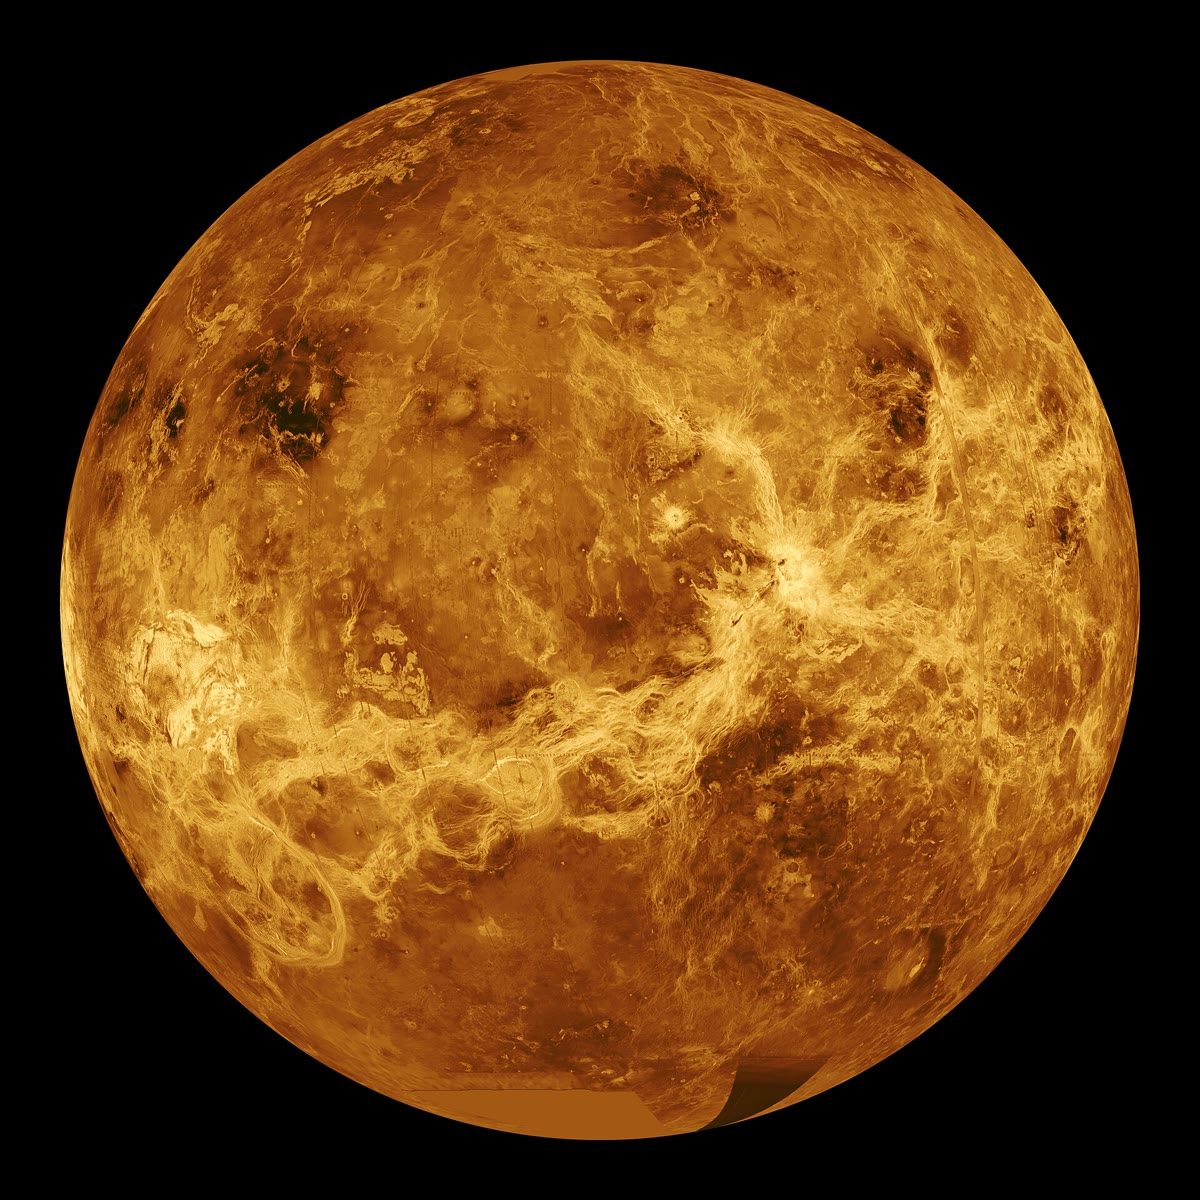
\includegraphics[width=\linewidth]{images/book3/b1-venus-radar-globe.jpg}
\end{minipage}\hspace{0.06\linewidth}
\begin{minipage}{0.4\linewidth}
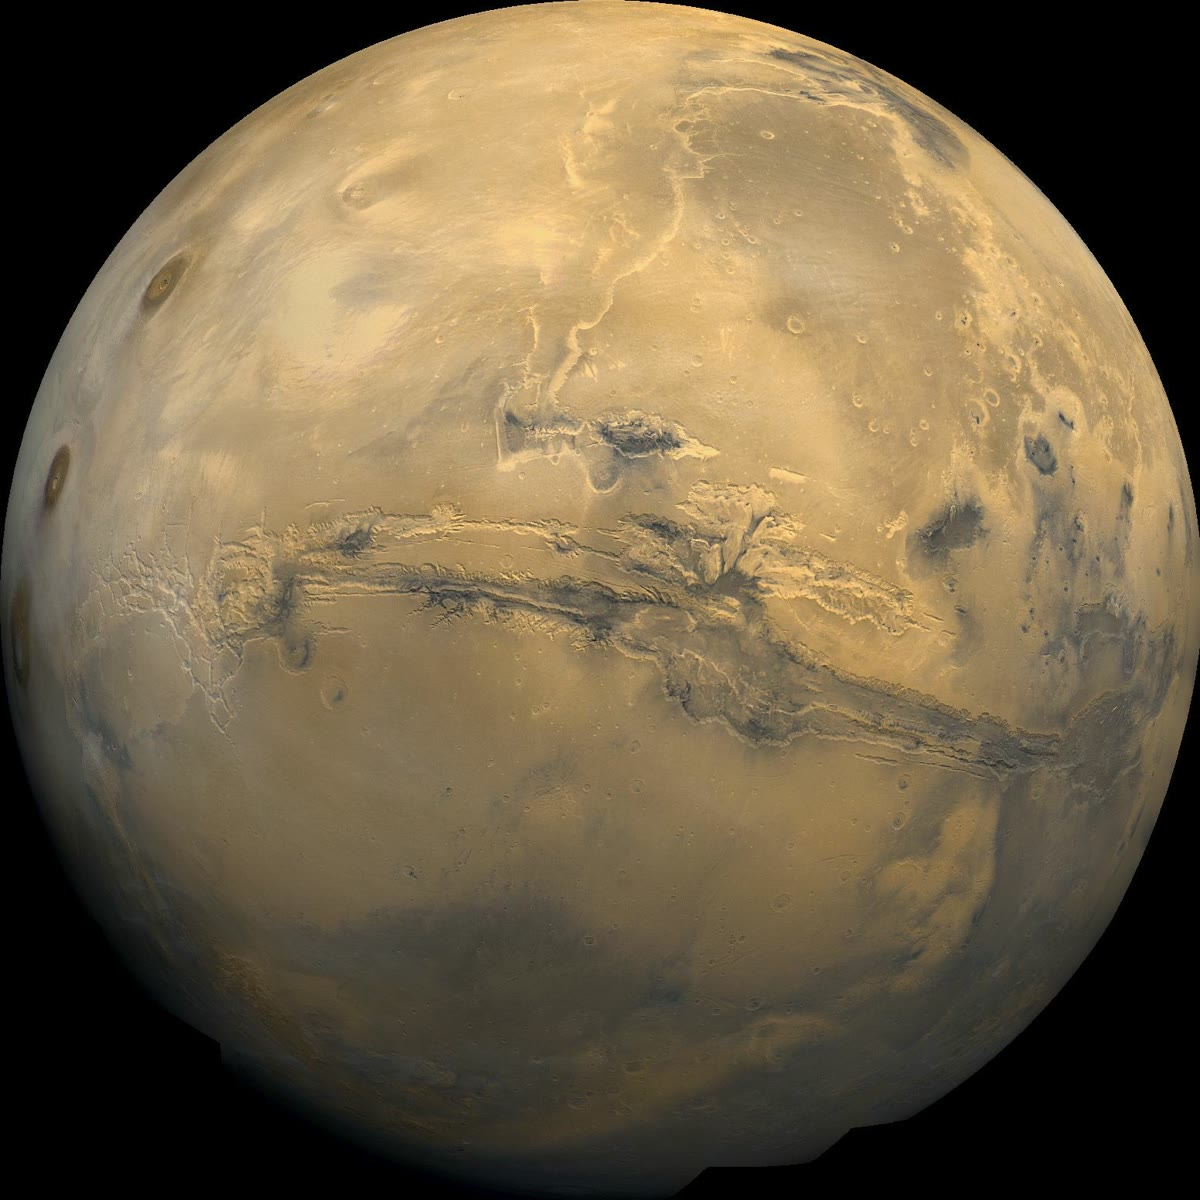
\includegraphics[width=\linewidth]{images/book3/b1-mars-valles-marineris.jpg}
\end{minipage}

{\small बाएँ: शुक्र की सतह, जैसी वह अपने बादलों के आर-पार मैगेलन यान के रडार से दिखती है, एक कंप्यूटर-
सिमुलेटेड गोले पर मानचित्रित (रंग सिमुलेटेड हैं)। दाएँ: वाइकिंग 1 कक्षायान से मंगल, जो वैलेस मरीनेरिस
घाटी-तंत्र पर केंद्रित एक मोज़ेक है। NASA/JPL और NASA/USGS, सार्वजनिक क्षेत्र।}
% ledger: commons:venus-globe, commons:mars-valles
\end{omfigure}

सतहें उस अभिलेख को रखती हैं कि उन्हें किसने आकार दिया। अंतरिक्ष के सामने खुली किसी भी सतह पर
उल्का-गर्त जमा होते हैं, इसलिए घने गर्तों वाली सतह, जैसे चंद्रमा या बुध की अधिकांश सतह, प्राचीन है,
और कम गर्तों वाली सतह नवीकृत हुई है: लावा प्रवाह से, अपरदन से, या उन प्लेटों से जो पृथ्वी की
महासागरीय तली को वापस प्रावार में ले जाती हैं। ज्वालामुखी मैदान और ज्वालामुखी सभी शैल-ग्रहों पर
मिलते हैं। भ्रंश, दरारें और मुड़ी हुई पेटियाँ दिखाती हैं कि शुक्र और मंगल के स्थलमंडल विरूपित हुए हैं;
पर सभी ग्रहों में केवल पृथ्वी आज ऐसा स्थलमंडल दिखाती है जो प्लेटों में टूटा है, जो दृढ़ खंडों की तरह
चलती हैं, जहाँ वे बनती हैं वहाँ कटक हैं और जहाँ वे धँसती हैं वहाँ खाइयाँ। पृथ्वी अकेले में
प्लेट विवर्तनिकी क्यों है, इस पर अब भी चर्चा होती है; जल की उपस्थिति, जो चट्टानों को दुर्बल करती है,
उन कारणों में से एक है जो सुझाए गए हैं।

\section{चंद्रमा और छोटे पिंड}

चंद्रमा, पृथ्वी के व्यास का एक चौथाई, एक उपग्रह के लिए बड़ा है। उसका घनत्व \qty{3340}{kg.m^{-3}}, जो
पृथ्वी के प्रावार की चट्टानों के निकट है, और उसका \omterm{def:b1:comparative-planetology:moi}{जड़त्व-आघूर्ण गुणक}, जो $0.4$ के निकट है, दिखाते हैं
कि उसमें अधिक-से-अधिक एक छोटा लौह-क्रोड है। विशाल ग्रहों के उपग्रह-तंत्र हैं जो अपने आप में संसार
हैं (नीचे के चित्र देखिए)। आयो, बृहस्पति के चार बड़े चंद्रमाओं में सबसे भीतरी, सौरमंडल का सबसे
अधिक ज्वालामुखी-सक्रिय संसार है, जिसमें सैकड़ों ज्वालामुखी हैं, और जिसे बृहस्पति द्वारा उसमें उठाए
गए ज्वारों से गर्म किया जाता है; ज्वालामुखीय क्रिया उसकी सतह को इतनी तेज़ी से नवीकृत करती है कि
प्रभाव बड़े गर्तों से उसे चिह्नित नहीं कर पाते। यूरोपा, जिसका घनत्व \qty{3010}{kg.m^{-3}} है, एक हिम
की भूपर्पटी के नीचे चट्टान है, और उस भूपर्पटी के नीचे एक खारे महासागर के लिए प्रबल प्रमाण हैं।
गैनीमीड और कैलिस्टो, जिनके घनत्व \num{1940} और \qty{1830}{kg.m^{-3}} हैं, तुलनीय मात्रा में चट्टान
और हिम से बने हैं। टाइटन, शनि का सबसे बड़ा चंद्रमा, अकेला ऐसा चंद्रमा है जिसका वायुमंडल सघन है, जो
मुख्यतः नाइट्रोजन और थोड़ी मीथेन से बना है, और पृथ्वी के अलावा अकेला ऐसा संसार है जिसकी सतह पर
नदियाँ, झीलें और समुद्र हैं --- द्रव मीथेन और ईथेन के; उसके नीचे भी संभवतः जल का एक महासागर छिपा है।
% ledger: planet:Moon.diameter, planet:Earth.diameter, planet:Moon.density, nasa:moon, nasa:io-facts, nasa:europa, nasa:europa-facts, nasa:ganymede, nasa:titan-facts

\begin{omfigure}
\begin{minipage}{0.4\linewidth}
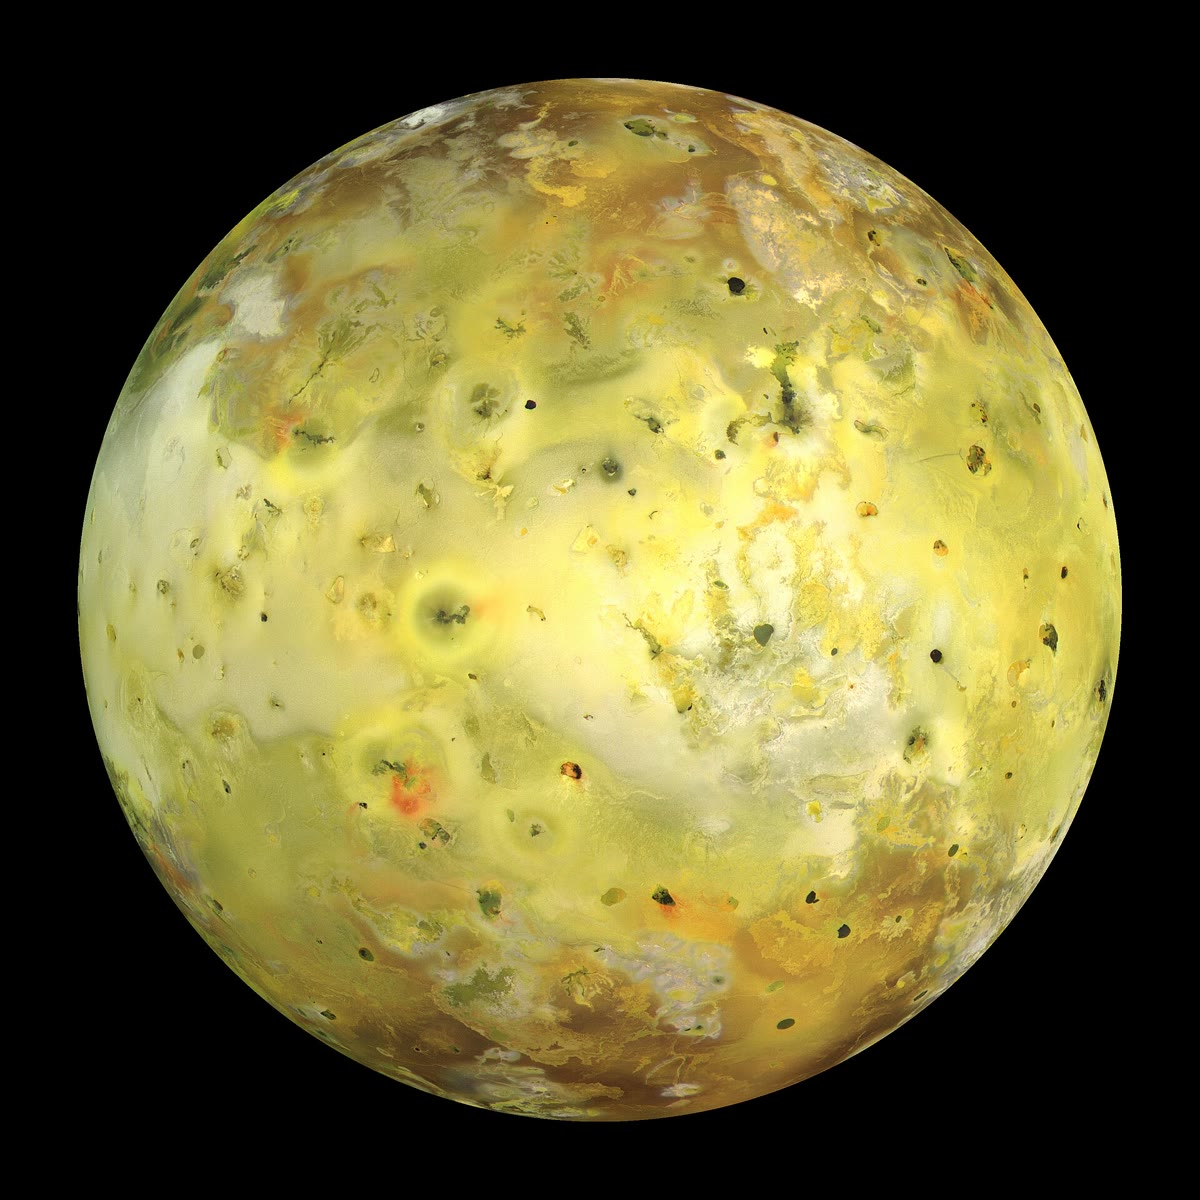
\includegraphics[width=\linewidth]{images/book3/b1-io.jpg}
\end{minipage}\hspace{0.06\linewidth}
\begin{minipage}{0.4\linewidth}
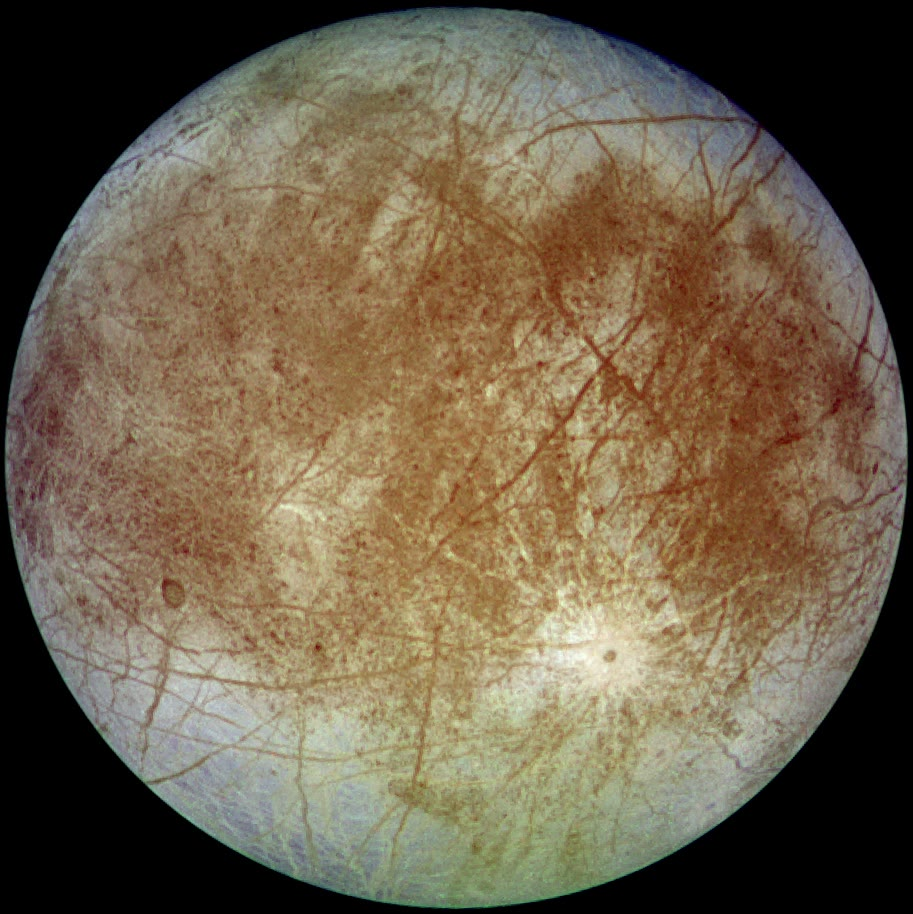
\includegraphics[width=\linewidth]{images/book3/b1-europa.jpg}
\end{minipage}

{\small बृहस्पति के दो बड़े चंद्रमा, गैलीलियो यान द्वारा देखे गए। बाएँ: आयो, जिसकी सतह ज्वालामुखी केंद्रों से
बिंदुकित है और गंधक यौगिकों तथा लावा से रंगी है। दाएँ: यूरोपा, लगभग प्राकृतिक रंग में; लंबी गहरी रेखाएँ
उसकी हिम-भूपर्पटी में दरारें हैं। NASA/JPL/ऐरिज़ोना विश्वविद्यालय और NASA/JPL/DLR, सार्वजनिक क्षेत्र।}
% ledger: commons:io, commons:europa, nasa:io-facts, nasa:europa
\end{omfigure}

\begin{definition}[क्षुद्रग्रह, धूमकेतु, नेप्च्यून-पार पिंड]\label{def:b1:comparative-planetology:small-bodies}
एक \emph{क्षुद्रग्रह}\index{क्षुद्रग्रह} सूर्य की परिक्रमा करने वाला एक छोटा शैलीय या धात्विक पिंड है,
जो ग्रह होने के लिए बहुत छोटा है और जिसके पास धूमकेतु जैसा गैस और धूल का आवरण नहीं है; अधिकांश
मंगल और बृहस्पति के बीच परिक्रमा करते हैं। एक \emph{धूमकेतु}\index{धूमकेतु} हिम और धूल का एक छोटा
पिंड है जो, जब उसकी कक्षा उसे सूर्य के निकट लाती है, गैस और धूल छोड़ता है जो उसके चारों ओर एक
चमकीला आवरण और सूर्य से दूर इंगित पूँछें बनाते हैं। एक \emph{नेप्च्यून-पार पिंड}\index{नेप्च्यून-पार पिंड}
सौरमंडल का ऐसा पिंड है जिसकी कक्षा औसतन नेप्च्यून की कक्षा से परे है।
\end{definition}

नेप्च्यून से परे एक चकती के आकार का क्षेत्र, कुइपर पेटी, के \omterm{def:b1:comparative-planetology:small-bodies}{नेप्च्यून-पार पिंड} ग्रहों के बनने से बचे
हिम और शैलीय पिंड हैं; प्लूटो, जिसे 2006 से बौना ग्रह माना जाता है, उनमें से एक है। \omterm{def:b1:comparative-planetology:small-bodies}{क्षुद्रग्रह}
ऐसे क्षेत्र के मलबे हैं जहाँ कोई ग्रह नहीं बना। क्षुद्रग्रहों के टुकड़े, और चंद्रमा तथा मंगल के कुछ
टुकड़े, उल्कापिंडों के रूप में पृथ्वी पर गिरते हैं। अंतरिक्ष यानों द्वारा वापस लाए गए नमूनों के
अलावा ये ही दूसरे संसारों के वे नमूने हैं जो हमारे हाथ में हैं, और उनमें से कुछ सौरमंडल के बनने
के बाद से बहुत कम बदले हैं; उनके वर्ग, और पृथ्वी के संघटन तथा सौरमंडल की आयु के बारे में वे क्या
बताते हैं, पुस्तक 4 (स्नातक वर्ष 2) का विषय हैं।
% ledger: nasa:pluto-facts

\section{अभ्यास}

\begin{exercise}[$\star$]\label{exo:b1:comparative-planetology:1}
बृहस्पति का द्रव्यमान \qty{1898.13e24}{kg} और माध्य त्रिज्या \qty{69911}{km} है। उसका माध्य घनत्व
परिकलित कीजिए और उसकी तुलना पानी के घनत्व, \qty{1000}{kg.m^{-3}}, से कीजिए।
\end{exercise}

\begin{exercise}[$\star$]\label{exo:b1:comparative-planetology:2}
आकृति के घनत्वों और त्रिज्याओं का उपयोग करके बुध, शनि, अरुण और शुक्र को \omterm{def:b1:comparative-planetology:planet-types}{शैल-ग्रह}, \omterm{def:b1:comparative-planetology:planet-types}{गैस दानव} या
\omterm{def:b1:comparative-planetology:planet-types}{हिम दानव} के रूप में वर्गीकृत कीजिए, और हर चुनाव को उसकी त्रिज्या और घनत्व से उचित ठहराइए।
\end{exercise}

\begin{exercise}[$\star$]\label{exo:b1:comparative-planetology:3}
शुक्र को \qty{2601.3}{W.m^{-2}} प्राप्त होता है और उसका \omterm{def:b1:comparative-planetology:albedo}{बॉन्ड एल्बिडो} 0.77 है। उसका \omterm{def:b1:comparative-planetology:equilibrium-temperature}{साम्य तापमान}
परिकलित कीजिए। वह पृथ्वी से कम क्यों है, यद्यपि शुक्र सूर्य के अधिक निकट है?
\end{exercise}

\begin{exercise}[$\star$]\label{exo:b1:comparative-planetology:4}
चंद्रमा ($C = 0.394$), मंगल (0.366), पृथ्वी (0.3308), बृहस्पति (0.254) और शनि (0.210) को सबसे
एकसमान से सबसे केंद्रित तक क्रम में रखिए। यदि एक ग्रह का पूरा द्रव्यमान उसके केंद्र पर एक बिंदु में
होता, तो $C$ क्या होता?
\end{exercise}

\begin{exercise}[$\star\star$]\label{exo:b1:comparative-planetology:5}
टाइटन शनि की परिक्रमा $a = \qty{1221.87e3}{km}$ पर \num{15.945421} दिनों में करता है। शनि का द्रव्यमान
परिकलित कीजिए और उसकी तुलना सारणीबद्ध \qty{568.32e24}{kg} से कीजिए।
\end{exercise}

\begin{exercise}[$\star\star$]\label{exo:b1:comparative-planetology:6}
पृथ्वी को सूर्य से \qty{149.6e6}{km} पर \qty{1361}{W.m^{-2}} प्राप्त होता है। मंगल (\qty{228.0e6}{km}) और
बृहस्पति (\qty{778.5e6}{km}) पर विकिरण-तीव्रता परिकलित कीजिए, और सारणीबद्ध \qty{586.2}{W.m^{-2}} और
\qty{50.26}{W.m^{-2}} से तुलना कीजिए।
\end{exercise}

\begin{exercise}[$\star\star$]\label{exo:b1:comparative-planetology:7}
दिखाइए कि किसी दिए गए एल्बिडो के लिए $T_\mathrm{eq}$, $d^{-1/2}$ के अनुसार बदलता है। बृहस्पति के लिए $T_\mathrm{eq}$ परिकलित कीजिए, जहाँ
$S = \qty{50.26}{W.m^{-2}}$ और $A = 0.343$ है। यदि पता चले कि बृहस्पति
सूर्य से जितनी शक्ति सोखता है उससे अधिक विकिरित करता है, तो इसका उसके भीतरी भाग के बारे में क्या अर्थ होगा?
\end{exercise}

\begin{exercise}[$\star\star$]\label{exo:b1:comparative-planetology:8}
शुक्र (\qty{737}{K}), पृथ्वी (\qty{288}{K}) और मंगल (\qty{214}{K}) के हरितगृह तापन $T_\mathrm{surf} - T_\mathrm{eq}$
परिकलित कीजिए, पृथ्वी के लिए $A = 0.294$ लेते हुए। हर एक को $T_\mathrm{eq}$ के भाग के रूप में व्यक्त कीजिए।
\end{exercise}

\begin{exercise}[$\star\star$]\label{exo:b1:comparative-planetology:9}
एक समान गोले के लिए, पतले गोलीय कोशों के जड़त्व-आघूर्णों का समाकलन करके दिखाइए कि $C = 0.4$ है (त्रिज्या
$r$ और द्रव्यमान $\mathrm dm$ वाले एक कोश का $\mathrm dI = \tfrac23 r^2\,\mathrm dm$ है)। त्रिज्या $R$ के
एक खोखले कोश का मान क्या है?
\end{exercise}

\begin{exercise}[$\star\star\star$]\label{exo:b1:comparative-planetology:10}
बुध का $\bar\rho = \qty{5429}{kg.m^{-3}}$, $C = 0.35$ और त्रिज्या \qty{2439.7}{km} है। \qty{3300}{kg.m^{-3}}
के प्रावार घनत्व के साथ दो-परत मॉडल से उसकी क्रोड-त्रिज्या, क्रोड का घनत्व और क्रोड में उसके द्रव्यमान का
भाग ज्ञात कीजिए। बुध के बारे में क्या विलक्षण है?
\end{exercise}

\begin{exercise}[$\star\star\star$]\label{exo:b1:comparative-planetology:11}
एक वायुहीन पिंड का प्रतिरूप बनाइए जिसका दिवस-गोलार्ध एकसमान तापमान $T_1$ पर और रात्रि-गोलार्ध $T_2$
पर है, और जो मिलकर अवशोषित शक्ति विकिरित करते हैं। (क) दिखाइए कि यदि $T_1^4 + T_2^4 = 2T_\mathrm{eq}^4$
हो, तो माध्य तापमान $(T_1 + T_2)/2$ अधिक-से-अधिक $T_\mathrm{eq}$ है, और समता केवल तब जब
$T_1 = T_2$। (ख) चंद्रमा के लिए $T_\mathrm{eq} = \qty{270}{K}$ है; $T_2 = \qty{100}{K}$ लीजिए। $T_1$ और माध्य
तापमान परिकलित कीजिए।
\end{exercise}

\begin{exercise}[$\star\star\star$]\label{exo:b1:comparative-planetology:12}
शुक्र की त्रिज्या \qty{6051.8}{km}, सतही गुरुत्व \qty{8.9}{m.s^{-2}} और सतही दाब \qty{92}{bar} है। उसके
वायुमंडल का द्रव्यमान परिकलित कीजिए, उसकी तुलना पृथ्वी के \qty{5.1e18}{kg} से, और शुक्र के
द्रव्यमान \qty{4.8673e24}{kg} से कीजिए। तुलना क्या सुझाती है कि पृथ्वी का कार्बन डाइऑक्साइड कहाँ रखा है?
% ledger: earth:Matm, planet:Venus.gravity, nasa:venus
\end{exercise}

\section{समस्या: मंगल को तौलना और उसकी थाह लेना}

\begin{problem}[{सप्ताहांत समस्या --- मंगल का द्रव्यमान उसके चंद्रमा से, उसका घनत्व और तापमान, और उसके क्रोड का आकार}]
\label{pb:b1:comparative-planetology:1}
% ledger: nasa:phobos, nasa:mars, nasa:mars-core, const:G, const:sigma, earth:psurf, earth:gmean, planet:Mars.Prot, planet:Earth.density
% numbers computed in the scratch calculator calc/ch03.py from the rounded data
फ़ोबोस, मंगल का बड़ा चंद्रमा, \num{0.31891} दिनों में मंगल के केंद्र से \qty{9378}{km} की माध्य दूरी पर
परिक्रमा करता है। मंगल की माध्य त्रिज्या \qty{3389.5}{km}, घूर्णन-काल \qty{24.6}{h}, \omterm{def:b1:comparative-planetology:moi}{जड़त्व-आघूर्ण गुणक}
$C = 0.366$, \omterm{def:b1:comparative-planetology:albedo}{बॉन्ड एल्बिडो} 0.250 और माध्य सतही दाब \qty{6.36}{mbar} है; वह सूर्य से \qty{586.2}{W.m^{-2}}
प्राप्त करता है, और उसका माध्य सतही तापमान लगभग \qty{214}{K} है। फ़ोबोस का द्रव्यमान
\qty{1.06e16}{kg} है। $G = \qty{6.6743e-11}{m^3.kg^{-1}.s^{-2}}$ और
$\sigma = \qty{5.6704e-8}{W.m^{-2}.K^{-4}}$ लीजिए।

\medskip
\noindent\textbf{भाग I --- मंगल को तौलना।}
\begin{enumerate}
  \item फ़ोबोस के आवर्तकाल को सेकंड में बदलिए।
  \item मंगल के लिए $GM$ परिकलित कीजिए।
  \item मंगल का द्रव्यमान निकालिए।
  \item क्या फ़ोबोस के द्रव्यमान की उपेक्षा करना ठीक है?
  \item फ़ोबोस की कक्षीय चाल परिकलित कीजिए।
  \item फ़ोबोस के आवर्तकाल की मंगल के घूर्णन से तुलना कीजिए। फ़ोबोस मंगल के आकाश को किस दिशा में पार करता है?
\end{enumerate}

\medskip
\noindent\textbf{भाग II --- घनत्व और गुरुत्व।}
\begin{enumerate}[resume]
  \item मंगल का आयतन परिकलित कीजिए।
  \item उसका माध्य घनत्व \qty{10}{kg.m^{-3}} तक पूर्णांकित करके परिकलित कीजिए।
  \item उसकी तुलना पृथ्वी के \qty{5514}{kg.m^{-3}} से कीजिए। पृथ्वी अधिक सघन क्यों है, इसके दो कारण दीजिए।
  \item मंगल की सतह पर गुरुत्व परिकलित कीजिए।
  \item मंगल की सतह से पलायन-वेग परिकलित कीजिए।
\end{enumerate}

\medskip
\noindent\textbf{भाग III --- तापमान और वायुमंडल।}
\begin{enumerate}[resume]
  \item मंगल का \omterm{def:b1:comparative-planetology:equilibrium-temperature}{साम्य तापमान} परिकलित कीजिए।
  \item उसकी तुलना माध्य सतही तापमान से कीजिए। हरितगृह तापन कितना बड़ा है?
  \item मंगल के हर वर्ग मीटर के ऊपर वायुमंडल का द्रव्यमान परिकलित कीजिए, और उसकी तुलना पृथ्वी ($p = \qty{1014}{hPa}$,
        $g = \qty{9.82}{m.s^{-2}}$) से कीजिए।
  \item मंगल के वायुमंडल का कुल द्रव्यमान परिकलित कीजिए।
  \item मंगल का वायुमंडल \qty{95}{\percent} कार्बन डाइऑक्साइड है, फिर भी उसका हरितगृह तापन छोटा है। कारण सुझाइए।
\end{enumerate}

\medskip
\noindent\textbf{भाग IV --- मंगल का क्रोड।}
\begin{enumerate}[resume]
  \item यदि मंगल एकसमान होता तो $C$ क्या होता? मापा गया मान क्या बताता है?
  \item दो-परत वाले मंगल का माध्य घनत्व सापेक्ष क्रोड-त्रिज्या $x$, प्रावार घनत्व $\rho_m$ और क्रोड घनत्व
        $\rho_c$ के रूप में लिखिए।
  \item उसका \omterm{def:b1:comparative-planetology:moi}{जड़त्व-आघूर्ण गुणक} उन्हीं पदों में लिखिए।
  \item दिखाइए कि $x^2 = (\tfrac52C\bar\rho - \rho_m)/(\bar\rho - \rho_m)$।
  \item प्रश्न 8 के माध्य घनत्व और $\rho_m =
        \qty{3500}{kg.m^{-3}}$ के साथ $x$ और क्रोड घनत्व परिकलित कीजिए।
  \item मंगल के द्रव्यमान का कितना भाग उसके क्रोड में है?
  \item $\rho_m = 3450$ और \qty{3550}{kg.m^{-3}} के साथ प्रश्न 21 दोहराइए। मॉडल की सूक्ष्मता के बारे में आप क्या निष्कर्ष निकालते हैं?
  \item $\rho_m = \qty{3500}{kg.m^{-3}}$ वाले मॉडल से मंगल की क्रोड-त्रिज्या दीजिए, और उसकी तुलना ग्रहीय सारणी के \qty{1830}{km} से, तथा हाल के भूकंपीय परिणाम (\qty{1650}{km} से \qty{1675}{km}) से कीजिए।
\end{enumerate}
\end{problem}
